\documentclass[a4paper]{article}
\usepackage[utf8]{inputenc}
\usepackage{fullpage}
\usepackage{csquotes}
\usepackage[ngerman]{babel}
\usepackage{biblatex}
\usepackage{float}
\usepackage{graphicx}
\usepackage{subfigure}
\usepackage[format=plain,labelfont=bf,up]{caption}
\usepackage{hyperref}
\usepackage{minted}
\usemintedstyle{friendly}
\bibliography{documentation.bib}
\title{Impaired Vision \\ Ein Augmented-Reality-Simulator für Sehstörungen}
\author{Willi Schönborn}
\date{\today}
\begin{document}

\begin{figure}[H]
\centering

\includegraphics{beuth.png}
\maketitle
\end{figure}

\section*{Einleitung}
Als Teil der Lehrveranstaltung \textit{Multimediatechnik Vertiefung} an der \textit{Beuth Hochschule für Technik Berlin} soltel im Rahmen einer Semesterarbeit ein Projekt mit Bezügen zu den Bereichen Multimedia und Wahrnehmung entstehen. Das Ziel dieses Dokumentes ist es die Ideen, Konzepte sowie die Ergebnisse dieses Projektes vorzustellen.

\section*{Augmented Reality}
Unter \textit{Augmented Reality} versteht man die computergestützte Erweiterung der Realitätswahrnehmung \cite{WP-AR}. Es gibt diverse doch sehr ausschweifende Definitionen dieses Begriffs. Innerhalb dieses Dokumentes wird Augmented Reality als die visuelle Darstellung von Informationen verstanden, also die Ergänzung von Bildern oder Videos mit computergenerierten Zusatzinformationen oder virtuellen Objekten mittels Einblendung/Überlagerung \cite{WP-AR}. Abbildung \ref{augmented-reality} zeigt eine typische Anwendung der Prinzipien von Augmented Reality anhand einer Anwendung für Smartphones, die es erlaubt geographische Informationen über Objekte die sich im Sichtfeld des Betrachters befinden direkt über das Kamerabild zu legen. Mithilfe solcher Augmented-Reality-Anwendungen entsteht eine neuartige Wahrnehmung der Umgebung. Genau an dieser Stelle setzt die Idee dieses Projektes an: Eine ungewohnte Sicht auf gewohnte Dinge ermöglichen.

\begin{figure}[H]
\centering
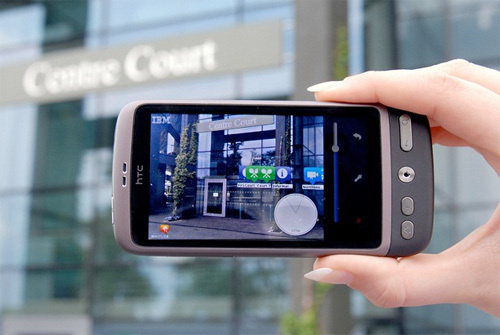
\includegraphics[width=\textwidth, trim=0 50 0 60, clip=true]{augmented-reality.jpg}
\caption{Augmented Reality Anwendung}
\label{augmented-reality}
\end{figure}

\newpage

\section*{Idee}
Die Projektidee ist eine Anwendung für Mobiltelefone, die es ermöglicht diverse Sehstörungen für normalsichtige Menschen zu simulieren. In der schriftlichen Projektidee wurden als mögliche Kandidaten für die Sehstörungen, die simuliert werden können Rot-Grün-Sehschwäche, Gelb-Blau-Sehschwäche sowie Kurzsichtigkeit aufgeführt. Nach einigen Recherchen sowie dem ausgiebigen Studium von \textit{Sensation and Perception} \cite{Goldstein2009} wurde relativ schnell deutlich, dass umgangssprachliche Vereinfachungen wie \textit{farbenblind} oder \textit{Rot-Grün-Schwäche} differenzierter betrachtet werden müssen um zu einem zufriedenstellenden Projektergebis zu kommen. Zu diesem Zweck werden im nächsten Kapitel alle Sehstörungen näher behandelt und analysiert, die später simuliert werden sollen.

\section*{Sehstörungen}
Insgesamt wurden fünf unterschiedliche Sehschwächen ausgewählt wobei der Schwerpunkt klar auf den Farbfehlsichtigkeiten liegt. Neben der klassischen Myopie, der Kurzsichtigkeit, sowie den drei Vertretern der Dichromasie, der teilweisen Farbblindheit \cite{WP-D} wird auch die Achromasie, die komplette Farbenblindheit, behandelt. Alle modifizierten Versionen der Beispielabbildungen in diesem Kapitel wurden mithilfe von Vischeck \cite{VISCHECK} erzeugt.

\subsection*{Myopie}
Kurzsichtigkeit oder Myopie bezeichnet man eine bestimmte Form von optischer Fehlsichtigkeit bei der ein Missverhältnis zwischen Baulänge und Brechkraft des Auges besteht. Das Ergebnis ist ein Abbildungsfehler, der weit entfernte Objekte unschärfer erscheinen lässt als nahe gelegene. Der Betroffene sieht also in der Ferne schlechter als in der Nähe \cite{WP-KS}. Abbildung \ref{myopia} verdeutlicht den Effekt anhand eines Fotos, das mit meinem Gauß-Filter \cite{WP-GF} modifiziert wurde. Die physikalische Grundlage ist hier nicht absolut korrekt, da bei der Kurzsichtigkeit natürlich die Entfernung eine große Rolle spielt, bei zunehmend großen Distanzen kann diese Tatsache jedoch vernachlässigt werden.

\begin{figure}[H]
\centering
\subfigure[Normalsichtigkeit]{
    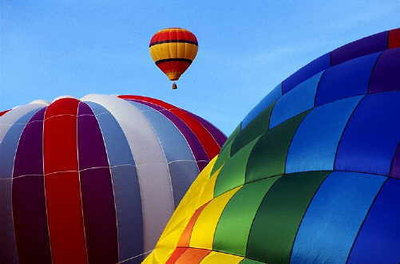
\includegraphics[width=0.48\textwidth]{balloons.jpg}
}
\subfigure[Myopie]{
    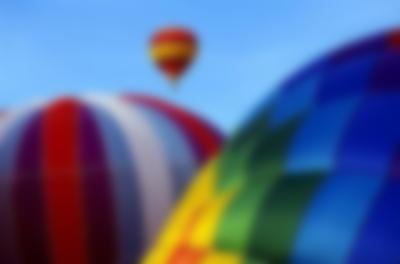
\includegraphics[width=0.48\textwidth]{balloons-myopia.jpg}
}
\caption{Myopie im Vergleich}
\label{myopia}
\end{figure}

\newpage

\subsection*{Protanopie}
Protanopie, oder auch Rotblindheit, ist einer Art der Dichromasie, also eine Farbsehstörung bei der nur zwei der drei Zapfen-Arten funktionsfähig sind. Bei Menschen mit Protanopie unterscheiden sich rote und grüne Zapfen nicht mehr in ihrer Farbantwort. Protanope haben daher nur zwei statt drei verschiedene Zapfentypen. Betroffen sind etwa 1 \% der Männer und 0,02 \% der Frauen. Im kurzwelligen Bereich sehen sie ein sattes Blau, im mittelwelligen Bereich Grau und im langwelligen Bereich ein sattes Gelb \cite{WP-P}.

\begin{figure}[H]
\centering
\subfigure[Normalsichtigkeit]{
    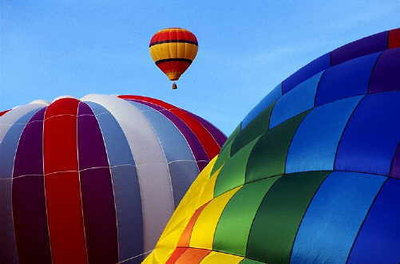
\includegraphics[width=0.48\textwidth]{balloons.jpg}
}
\subfigure[Protanopie]{
    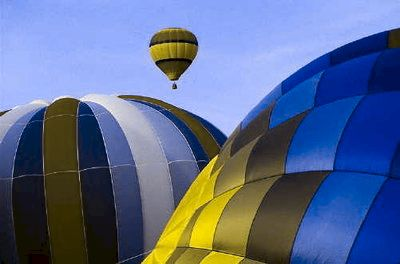
\includegraphics[width=0.48\textwidth]{balloons-protanope.jpg}
}
\caption{Protanopie im Vergleich}
\label{protanope}
\end{figure}

\subsection*{Deuteranopie}
Auch bei der Deuteranopie, oder Gründblindheit, handelt sich dabei um eine genetisch bedingte Farbfehlsichtigkeit Deuternaropen haben jedoch, im Gegensatz zu Protanopen, keine funktionsfähigen M-Zapfen da die Zapfen für das Wahrnehmen von Grün das Opsin für Rot enthalten \cite{WP-D}. Die Krankheitshäufigkeit von Deuteranopie liegt im selben Bereich wie die der Protanopie. Interessant ist die Tatsache, dass beide Krankheiten, sowohl die Rot- als auch die Grünblindheit, einen ausgesprochen ähnlichen visuellen Effekt ergeben. Betroffene können in beiden Fällen Rot- und Grüntöne der gleichen Helligkeit nicht mehr auseinanderhalten. Aus diesem Grund werden beide Krankheiten oft unter dem Begriff Rot-Grün-Sehschwäche \cite{WP-RG} zusammengefasst. Die Abbildung \ref{protanope} und \ref{deuteranope} zeigen die jeweiligen Symptome im direkten Vergleich mit der Normalsichtigkeit.

\begin{figure}[H]
\centering
\subfigure[Normalsichtigkeit]{
    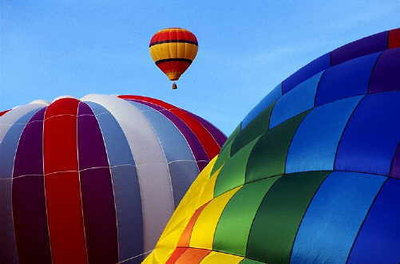
\includegraphics[width=0.48\textwidth]{balloons.jpg}
}
\subfigure[Deuteranopie]{
    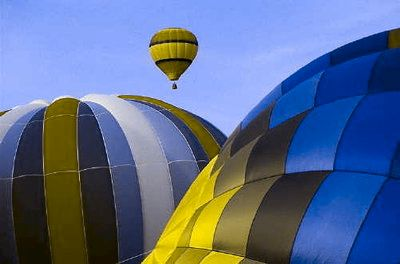
\includegraphics[width=0.48\textwidth]{balloons-deuteranope.jpg}
}
\caption{Deuteranopie im Vergleich}
\label{deuteranope}
\end{figure}

\newpage

\subsection*{Tritanopie}
Tritanopie, oder Blaublindheit, bezeichnet eine genetisch bedingte Farbfehlsichtigkeit, bei der den Betroffenen die Blau-Zapfen in der Retina fehlen \cite{WP-T}. Die Prävalenz von Tritanopie ist mit etwa 0,002 \% der Männer und 0,001 \% der Frauen verglichen mit Protanopie und Deuteranopie deutlich geringer. Die Tatsache, dass Betroffene keine Funktionsfähigen S-Zapfen haben führt dazu, dass mittlere und kurze Wellenlängen nicht mehr einwandfrei unterschieden werden können. Abbildung \ref{tritanope} verdeutlicht diesen Effekt.

\begin{figure}[H]
\centering
\subfigure[Normalsichtigkeit]{
    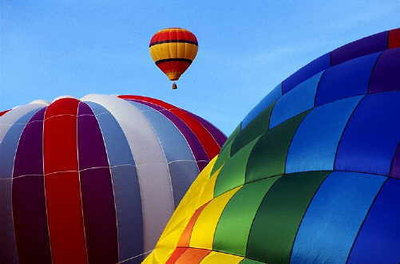
\includegraphics[width=0.48\textwidth]{balloons.jpg}
}
\subfigure[Tritanopie]{
    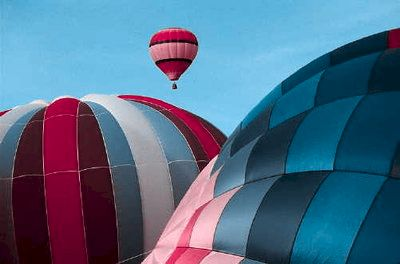
\includegraphics[width=0.48\textwidth]{balloons-tritanope.jpg}
}
\caption{Tritanopie im Vergleich}
\label{tritanope}
\end{figure}

\subsection*{Achromasie}
Die Farbenblindheit, Achromatopsie oder Achromasie ist eine seltene Farbsinnstörung, bei der keine Farben, sondern nur Hell-Dunkel-Kontraste wahrgenommen werden können. Bei Achromaten funktioniert keine der drei Zapfenarten, sie können somit keine Farben erkennen \cite{WP-A}. Neben der Unfähigkeit Farben zu erkennen leiden Achromaten zusätzlich darunter, dass im Bereich der Fovea keinerlei funktionierende Rezeptoren existieren. Dadurch fehlt ein Großteil der Sehschärfe. Abbildung \ref{achromate} versucht den visuellen Effekt mithilfe eines Graustufenbildes und eines Gauß-Filters zu simulieren. Allerdings lässt sich der visuelle Eindruck für Normalsichtige nicht zuverlässig darstellen. Diese Abbildung sollte deshalb nur als mögliche Interpretation verstanden werden.

\begin{figure}[H]
\centering
\subfigure[Normalsichtigkeit]{
    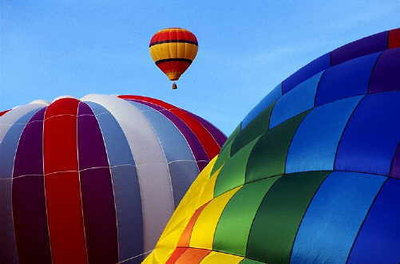
\includegraphics[width=0.48\textwidth]{balloons.jpg}
}
\subfigure[Achromasie]{
    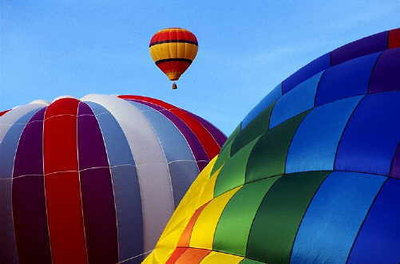
\includegraphics[width=0.48\textwidth]{balloons-achromate.jpg}
}
\caption{Achromasie im Vergleich}
\label{achromate}
\end{figure}

\newpage

\section*{Implementierung}
Der Simulator wurde auf Basis der Android Plattform 2.3.3 entwickelt. Als Testgerät kam das \textit{Google Nexus S} zum Einsatz. Ein wichtiger Beweggrund für die Wahl der Plattform war die persönliche Vorliebe des Autors für die Programmiersprache Java sowie die überaus umfangreiche Dokumentation der Android API. Für die Implementierung der verschiedenen Sehstörungen waren  unterschiedliche Vorgehensweise nötig die in den folgenden Abschnitten genauer erklärt werden. Alle Bilder, die Ergebnisse bestimmter Effekte zeigen, sind ausschließlich mit dem entwickelten Simulator entstanden und wurden nachträglich in keiner Weise manipuliert.

\subsection*{Kurzsichtigkeit}
Die erste naive Idee Myopie zu simulieren war das Modifizieren des Kamerabildes mithilfe eines Gauß-Filters. Bei diesem Ansatz wird allerdings vernachlässigt, dass Betroffene in einem kleinen Bereich, abhängig der tatsächlichen Sehstärke, durchaus scharf sehen können. Aus diesem Grund wurde von diesem Ansatz Abstand genommen. Stattdessen wurde ein einfacheres und dennoch korrektes Verfahren implementiert: Kameras in Android-gestützten Mobiltelefonen verfügen über einen Auto-Fokus der jedoch programmatisch deaktiviert werden kann. Statt dem Auto-Fokus kann ein statischer Fokus festgelegt werden. Für die Simulation von Kurzsichtigkeit bietet sich hier natürlich der Makro-Fokus an. Diese Technik hat den Vorteil, dass Objekte die sich in kurzer Entfernung zum Betrachter befinden scharf gesehen werden können während mit zunehmender Entfernung Details nicht mehr wahrgenommen werden können. Leider ist der Makro-Fokus statisch, das heißt die Entfernung ab der Unschärfe zu sehen ist lässt sich nicht einstellen. Auf dem Testgerät war der visuelle Eindruck ausgesprochen nah an der tatsächlichen Sehstärke des Autors, die nach letzten Messungen im Bereich um 6,75 Dioptrin liegt. Listing \ref{macro-focus} zeigt die Aktivierung des Makro-Fokus mithilfe der Android-Klasse \texttt{android.hardware.Camera}.

\begin{listing}[H]
\begin{minted}{java}
@Override
public void configure(Camera camera) {
    final Camera.Parameters parameters = camera.getParameters();
    parameters.setFocusMode(Camera.Parameters.FOCUS_MODE_MACRO);
    camera.setParameters(parameters);
}
\end{minted}
\caption{Aktivierung des Makro-Fokus}
\label{macro-focus}
\end{listing}

Abbildung \ref{simulated-myopia} zeigt das Ergebnis dieser Implementierung anhand eines Screenshots von der laufenden Anwendung der mit Mithilfe des Android Tools \textit{Dalvik Debug Monitor Server} erstellt wurde.

\begin{figure}[H]
\centering
\subfigure[Normalsichtigkeit]{
    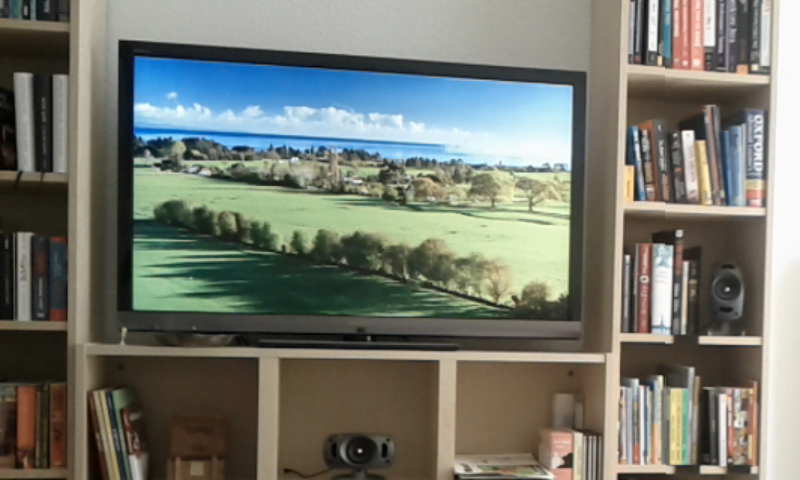
\includegraphics[width=0.48\textwidth]{normal.png}
}
\subfigure[Myopie]{
    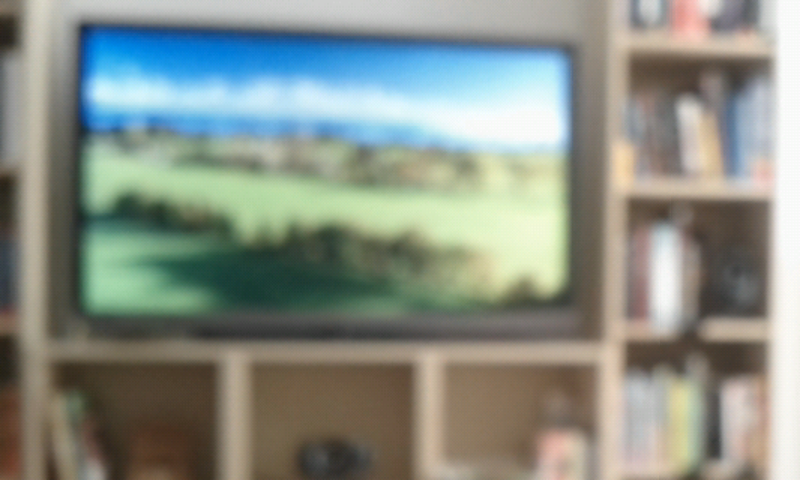
\includegraphics[width=0.48\textwidth]{myopia.png}
}
\caption{Simulierte Kurzsichtigkeit}
\label{simulated-myopia}
\end{figure}

\newpage

\subsection*{Farbfehlsichtigkeiten}
Im Gegensatz zur Kurzsichtigkeit wurden die restlichen Farbsehstörungen durch direkte Manipulation des Kamerabildes realisiert. Dazu muss eine Instanz der Schnittstelle \texttt{android.hardware.Camera.PreviewCallback}, wie in Listing \ref{preview-register} zu sehen ist, implementiert und bei der aktuellen \texttt{Camera} registriert werden.

\begin{listing}[H]
\begin{minted}{java}
@Override
public void onPreviewFrame(byte[] frame) {
     ...
}

@Override
public void surfaceCreated(SurfaceHolder holder) {
    camera.setPreviewCallback(this);
}
\end{minted}
\caption{Implementierung und Registrierung eines PreviewCallbacks}
\label{preview-register}
\end{listing}

In der \texttt{onPreviewFrame}-Methode hat man nun Zugriff auf den aktuellen Frame in Form eines Byte-Arrays das die Bildinformationen im NV21-Byteformat enthält, einer Variante von YCbCr/YUV 4:2:0 wobei die beiden Farbanteile in der Reihenfolge vertauscht werden. Im ersten Schritt muss das Bild also in den RGB-Farbraum konvertiert werden. Dieser Schritt wurde mit dem Algorithmus von David Manpearl realisiert, der unter \cite{ANDROID-YUV} zu finden ist. Auf die entstandene RGB-Bitmap können nun Farbeffekte angewendet werden. Für diesen Zweck kommt die Android-Klasse \texttt{android.graphics.ColorMatrixColorFilter} zum Einsatz. Diese Filter werden als 5x4-Matrizen deklariert und definieren eine Abbildung zwischen den Farbwerten der eingehenden Pixel und der Ergebnisfarbe. Das folgende Listing \ref{matrix-protanopia} und die Abbildung \ref{simulated-protanopia} zeigen die Konfiguration eines \texttt{ColorMatrixColorFilter}s anhand der Protanopie sowie den erzeugten Effekt.

\begin{listing}[H]
\begin{minted}{java}
new ColorMatrixColorFilter(new float[] {
    0.567f, 0.433f, 0.0f, 0.0f, 0.0f,
    0.558f, 0.442f, 0.0f, 0.0f, 0.0f,
    0.0f, 0.242f, 0.758f, 0.0f, 0.0f,
    0.0f, 0.0f, 0.0f, 1.0f, 0.0f,
});
\end{minted}
\caption{Konfiguration eines ColorMatrixColorFilters}
\label{matrix-protanopia}
\end{listing}

\begin{figure}[H]
\centering
\subfigure[Normalsichtigkeit]{
    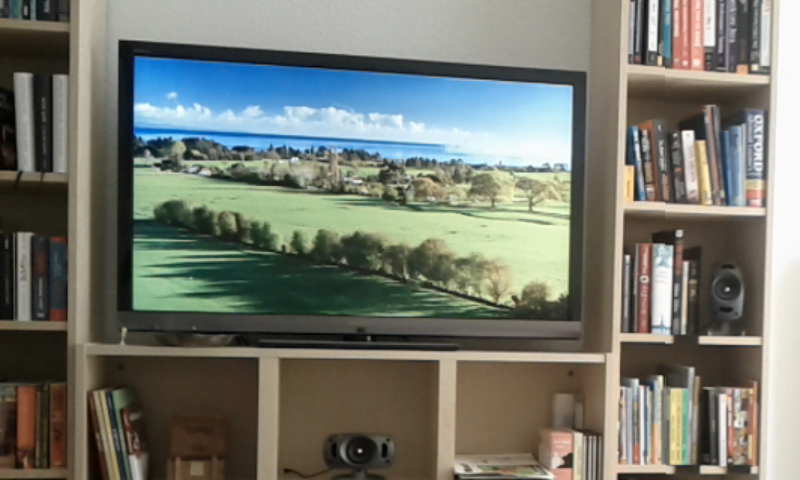
\includegraphics[width=0.48\textwidth]{normal.png}
}
\subfigure[Protanopie]{
    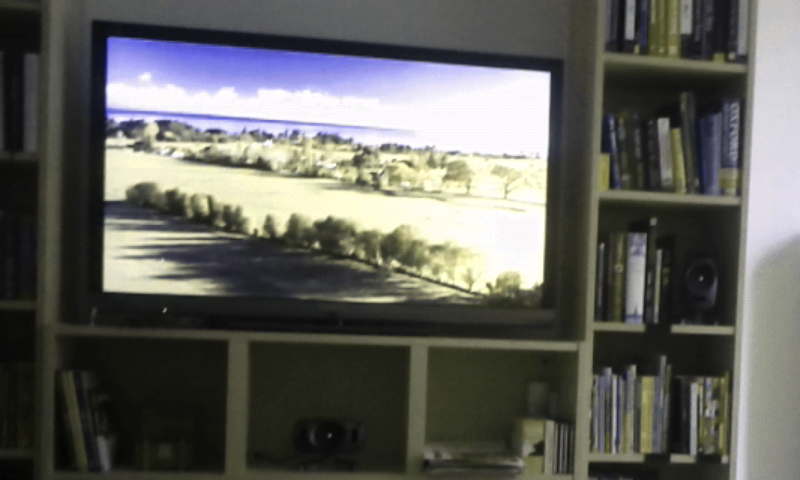
\includegraphics[width=0.48\textwidth]{protanopia.png}
}
\caption{Simulierte Protanopie}
\label{simulated-protanopia}
\end{figure}

Der Helligkeitsunterschied zwischen der Normalsichtigkeit und der Protanopie ist nicht bedingt durch den Farbfilter sondern durch die Tatsache, dass beide Bilder zu unterschiedlichen Tageszeiten aufgenommen wurden und dementsprechend der Grad an Sonneneinstrahlung unterschiedlich war.

Die folgenden Abbildungen zeigen die simulierten Effekte für die restlichen Sehstörungen.

\begin{figure}[H]
\centering
\subfigure[Normalsichtigkeit]{
    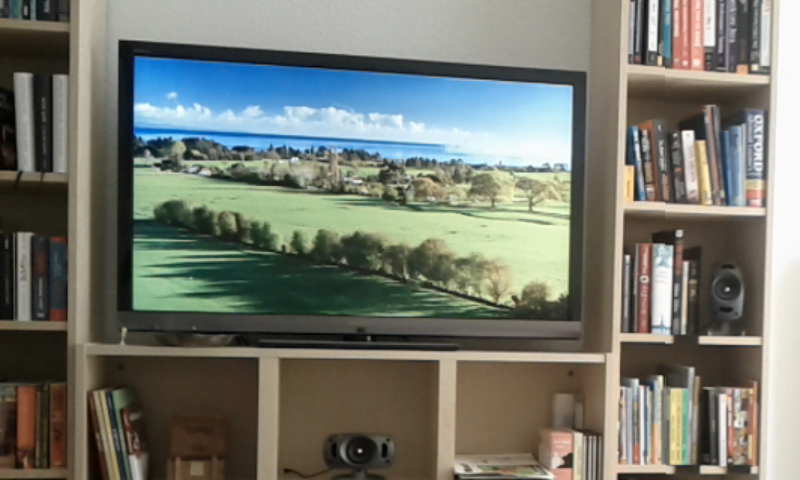
\includegraphics[width=0.48\textwidth]{normal.png}
}
\subfigure[Deuteranopie]{
    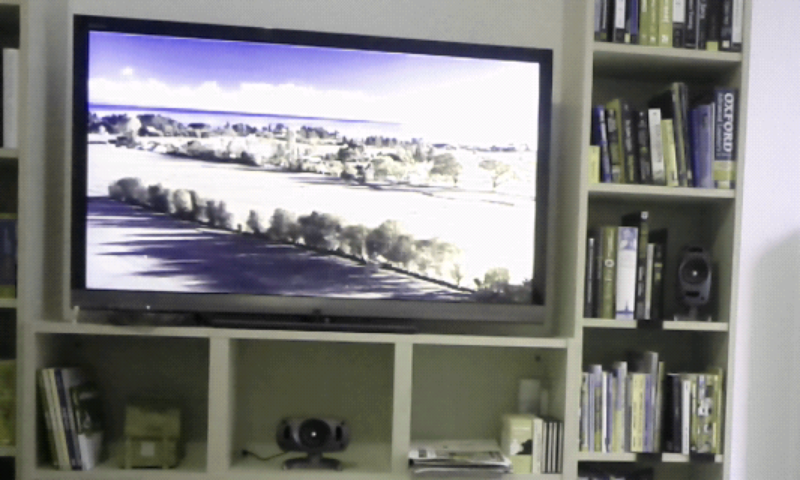
\includegraphics[width=0.48\textwidth]{deuteranopia.png}
}
\caption{Simulierte Deuteranopie}
\end{figure}

\begin{figure}[H]
\centering
\subfigure[Normalsichtigkeit]{
    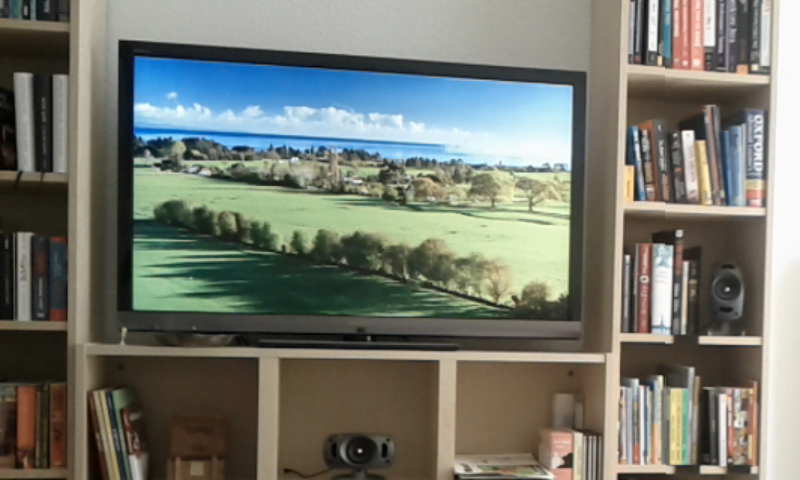
\includegraphics[width=0.48\textwidth]{normal.png}
}
\subfigure[Tritanopie]{
    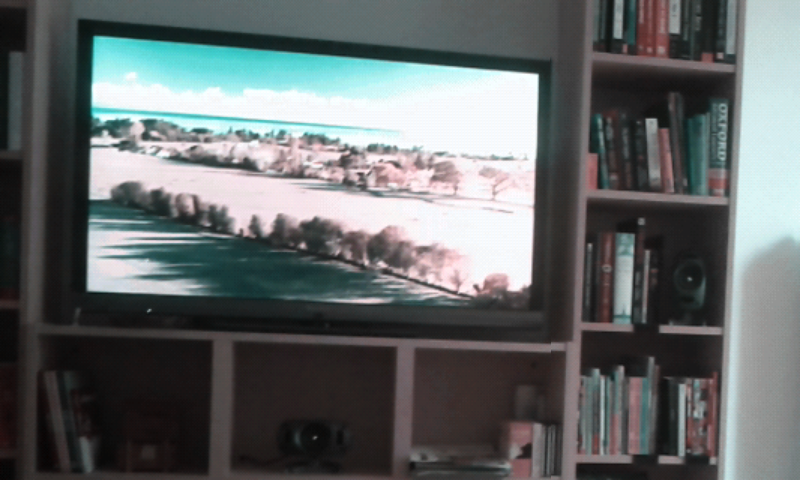
\includegraphics[width=0.48\textwidth]{tritanopia.png}
}
\caption{Simulierte Tritanopie}
\end{figure}

\begin{figure}[H]
\centering
\subfigure[Normalsichtigkeit]{
    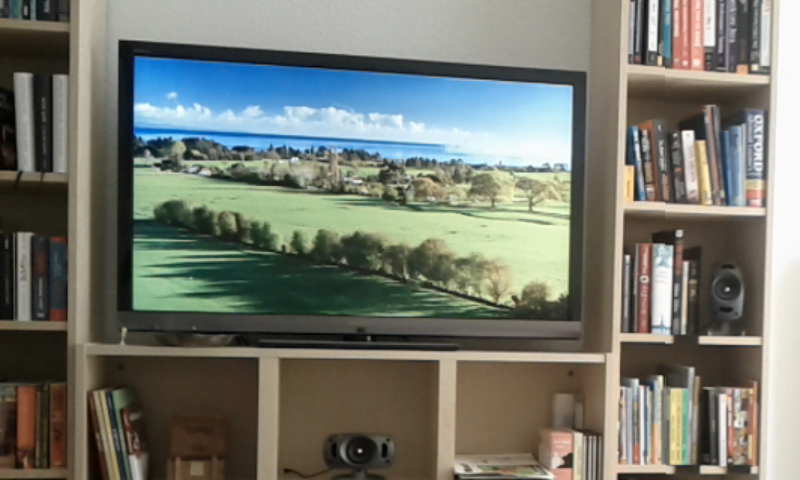
\includegraphics[width=0.48\textwidth]{normal.png}
}
\subfigure[Achromasie]{
    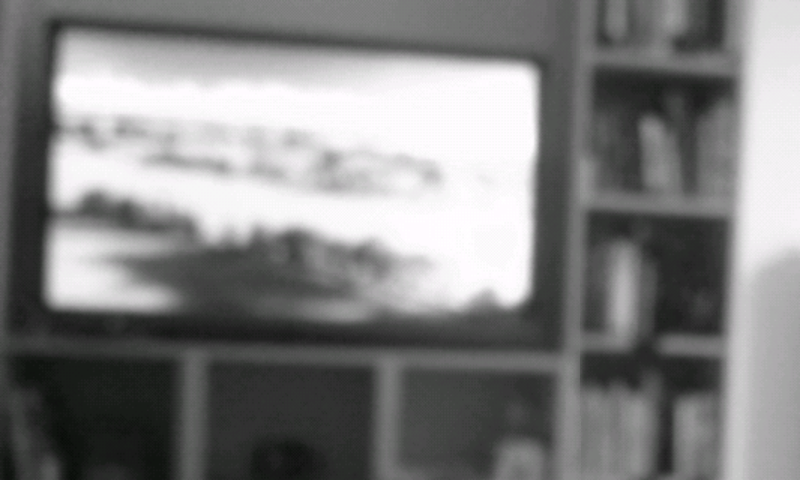
\includegraphics[width=0.48\textwidth]{achromatopia.png}
}
\caption{Simulierte Achromasie}
\end{figure}

\newpage

\subsection*{Geschwindigkeit und Optimierungen}
Ohne zusätzliche Konfiguration haben eingehende Bilder der Kamera auf einem \textit{Google Nexus S} eine Auflösung von 720x480 Pixel bei einer durchschnittlichen Framerate von 15 - 30 Bildern pro Sekunde.

\newpage

\nocite{ANDROID}
\nocite{GIZMODO}
\nocite{IBFB}
\printbibliography

\listoffigures

\renewcommand\listoflistingscaption{Quellcodeverzeichnis}
\listoflistings

\end{document}

